%
% $RCSfile: knowledge_abstraction_and_manipulation.tex,v $
%
% Copyright (C) 2002-2008. Christian Heller.
%
% Permission is granted to copy, distribute and/or modify this document
% under the terms of the GNU Free Documentation License, Version 1.1 or
% any later version published by the Free Software Foundation; with no
% Invariant Sections, with no Front-Cover Texts and with no Back-Cover
% Texts. A copy of the license is included in the section entitled
% "GNU Free Documentation License".
%
% http://www.cybop.net
% - Cybernetics Oriented Programming -
%
% http://www.resmedicinae.org
% - Information in Medicine -
%
% Version: $Revision: 1.1 $ $Date: 2008-08-19 20:41:07 $ $Author: christian $
% Authors: Christian Heller <christian.heller@tuxtax.de>
%

\section{Knowledge Abstraction and -Manipulation}
\label{knowledge_abstraction_and_manipulation_heading}
\index{Knowledge Abstraction}
\index{Knowledge Manipulation}

Having shown the existence of state- and logic knowledge, not only in software
systems, and having compared both with a classical layered software architecture,
what is still missing is an overview of fundamental abstractions of state- as
well as logic knowledge, and a solution showing how both can be manipulated, in
a knowledge-based system.

%
% $RCSfile: algorithm.tex,v $
%
% Copyright (C) 2002-2008. Christian Heller.
%
% Permission is granted to copy, distribute and/or modify this document
% under the terms of the GNU Free Documentation License, Version 1.1 or
% any later version published by the Free Software Foundation; with no
% Invariant Sections, with no Front-Cover Texts and with no Back-Cover
% Texts. A copy of the license is included in the section entitled
% "GNU Free Documentation License".
%
% http://www.cybop.net
% - Cybernetics Oriented Programming -
%
% http://www.resmedicinae.org
% - Information in Medicine -
%
% Version: $Revision: 1.1 $ $Date: 2008-08-19 20:41:05 $ $Author: christian $
% Authors: Christian Heller <christian.heller@tuxtax.de>
%

\subsection{Algorithm}
\label{algorithm_heading}
\index{Algorithm}
\index{Knowledge Engineering}
\index{KE}
\index{Ontology}
\index{Knowledge Schema}
\index{State Model}
\index{Logic Model}
\index{Sequence of (Mapping) Rules}
\index{Lambda Calculus}
\index{Turing Machine}

For John F. Sowa \cite{sowa}, \emph{Knowledge Engineering} (KE) is:
\textit{the application of logic and ontology to the task of building
computable models of some domain for some purpose.} Section
\ref{knowledge_representation_heading} showed how an \emph{Ontology} can be
applied to structure state knowledge of a domain, and introduced a new
\emph{Knowledge Schema}. This section investigates the universality of that
knowledge schema, that is its applicability to \emph{State-} as well as
\emph{Logic} models.

Not only input/ output (i/o) knowledge (states) can be structured
hierarchically, using an ontology, the operations of a system (logic) can be
cascaded and nested as well. The resulting logic models are \emph{Sequences} of
input-to-output mapping rules that can consist of yet finer-grained models. The
theory of computing uses the word \emph{Algorithm} to label a sequence of
mapping rules. Banerjee \cite{banerjee} writes on this:

\begin{quote}
    Each \ldots\ mathematician had to precisely define the notion of an
    algorithm, and each defined it in a different way. Godel defined algorithm
    as a \emph{Sequence of Rules} for forming complicated mathematical
    functions out of simple mathematical functions, Church used a formalism
    called the \emph{Lambda Calculus}, while Turing used a mathematical object
    called the \emph{Turing Machine} and defined an algorithm to be any set of
    instructions for his simple machine. All these seemingly different and
    independently contrived definitions turned out to be equivalent and they
    form the basics of the modern theory of computing. No modern programming
    language can achieve more, in principle, than the Turing machine or the
    lambda-calculus.
\end{quote}

\emph{Time} plays an important role in data processing. It dictates the order
in which steps of an algorithm are executed and thereby ensures a correct
sequence of actions. Every element of an algorithm needs to be assigned an
instant (position) in time, as meta information. Although the runtime-processing
of data, according to an algorithm, is \emph{dynamic}, the models of logic --
just like i/o state models -- are \emph{static} (chapter
\ref{statics_and_dynamics_heading}).

%
% $RCSfile: operations.tex,v $
%
% Copyright (C) 2002-2008. Christian Heller.
%
% Permission is granted to copy, distribute and/or modify this document
% under the terms of the GNU Free Documentation License, Version 1.1 or
% any later version published by the Free Software Foundation; with no
% Invariant Sections, with no Front-Cover Texts and with no Back-Cover
% Texts. A copy of the license is included in the section entitled
% "GNU Free Documentation License".
%
% http://www.cybop.net
% - Cybernetics Oriented Programming -
%
% http://www.resmedicinae.org
% - Information in Medicine -
%
% Version: $Revision: 1.1 $ $Date: 2008-08-19 20:41:08 $ $Author: christian $
% Authors: Christian Heller <christian.heller@tuxtax.de>
%

\subsection{Operations}
\label{operations_heading}
\index{Operation}
\index{Binary Arithmetic}
\index{Digital Logic Circuit}
\index{Two's Complement}
\index{AND Operation}
\index{Boolean Operation}
\index{Comparison Operation}
\index{Arithmetic Operation}

In the end, all computer-implemented procedures go back to boolean operations
and binary arithmetic (section \ref{from_philosophy_to_mathematics_heading}),
processed by digital logic circuits (section \ref{digital_logic_heading}). A
\emph{Multiplication} can be expressed as sequence of additions. By
representing the number to be subtracted in its negative form
(\emph{Two's Complement} \cite{philippow}), a \emph{Subtraction} can be mapped
to an addition. An \emph{Addition} itself is performed by linking Bits of the
summands logically, using an \emph{AND} operation. Fundamental operations for
knowledge translation are:

\begin{itemize}
    \item[-] \emph{Boolean:} and, or
    \item[-] \emph{Comparison:} equal, smaller, greater
    \item[-] \emph{Arithmetic:} add, subtract, multiply, divide
\end{itemize}

They all imply special rules after which one or more input operands (values)
get transformed into one or more output operands. Both kinds representing
static \emph{State Models}, input and output can be placed as branches of one
common knowledge tree. But also the rules as static \emph{Logic Models} can be
added to this tree.

%
% $RCSfile: primitives.tex,v $
%
% Copyright (C) 2002-2008. Christian Heller.
%
% Permission is granted to copy, distribute and/or modify this document
% under the terms of the GNU Free Documentation License, Version 1.1 or
% any later version published by the Free Software Foundation; with no
% Invariant Sections, with no Front-Cover Texts and with no Back-Cover
% Texts. A copy of the license is included in the section entitled
% "GNU Free Documentation License".
%
% http://www.cybop.net
% - Cybernetics Oriented Programming -
%
% http://www.resmedicinae.org
% - Information in Medicine -
%
% Version: $Revision: 1.1 $ $Date: 2008-08-19 20:41:08 $ $Author: christian $
% Authors: Christian Heller <christian.heller@tuxtax.de>
%

\subsection{Primitives}
\label{primitives_heading}
\index{Primitive}
\index{State Primitive}
\index{Binary Digit}
\index{Bit}
\index{Byte}
\index{Word}
\index{Double Word}
\index{File}
\index{Hard Disk Drive}
\index{HDD}
\index{Random Access Memory}
\index{RAM}
\index{Multipurpose Internet Mail Extension}
\index{MIME}
\index{Text MIME Type}
\index{Image MIME Type}
\index{Audio MIME Type}
\index{Video MIME Type}
\index{Application MIME Type}

All software is based on the final two states called \emph{one} \& \emph{zero},
or \emph{on} \& \emph{off}, or \emph{true} \& \emph{false}, or similarly. A
\emph{Binary Digit} (Bit) can take on the values \emph{zero} or \emph{one}; it
represents the final abstraction of any software model and can be easily mapped
to hardware. A second unit, the \emph{Byte}, consists of eight Bits. One
\emph{Word} is made up of two Bytes, one \emph{Double Word} of four Bytes and
so forth. Data in a \emph{File} on a \emph{Harddisk Drive} (HDD) partition or
another storage medium are saved in form of Bit sequences, just like data in
\emph{Random Access Memory} (RAM). It is up to a program to interpret these
data correctly, in the desired manner.

\begin{figure}[ht]
    \begin{center}
        \begin{footnotesize}
        \begin{tabular}{| p{70mm} | p{35mm} |}
            \hline
            \textbf{Primitivum} & \textbf{Size} [Byte]\\
            \hline
            Date, Time, Complex, Fraction, Term & many\\
            \hline
            Double, Float, Vector, String & 8, 12, 16 or more\\
            \hline
            Integer, Pointer, Word, Short, Byte, Character & 1, 2, 4, 7, 8 or more\\
            \hline
            Bit, Boolean & 0 or 1 Bit\\
            \hline
        \end{tabular}
        \end{footnotesize}
        \caption{State Primitives sorted after their Granularity}
        \label{primitives_table}
    \end{center}
\end{figure}

Many programming languages offer a number of basic types, also called
\emph{Primitives}, which are combinations of different numbers of Bits. Table
\ref{primitives_table} shows some of them, together with their possible memory
usage. Besides the primitive types that are included in a programming language,
there are other forms of storing data. Section \ref{language_heading} said that
not only a \emph{String}, but also an \emph{Image} or a \emph{Sound} can
represent a \emph{Quality}, that is a \emph{Term} with special meaning. The
format of such data sequences is often defined as
\emph{Multipurpose Internet Mail Extension} (MIME) type, for example:

\begin{itemize}
    \item[-] \emph{text:} sgml, xml, html, rtf, tex, txt
    \item[-] \emph{image:} jpeg, png, gif, bmp
    \item[-] \emph{audio:} ogg, mp3, wav
    \item[-] \emph{video:} mpeg, qt, avi
    \item[-] \emph{application:} kword, sxw
\end{itemize}

%
% $RCSfile: logic_manipulates_state.tex,v $
%
% Copyright (C) 2002-2008. Christian Heller.
%
% Permission is granted to copy, distribute and/or modify this document
% under the terms of the GNU Free Documentation License, Version 1.1 or
% any later version published by the Free Software Foundation; with no
% Invariant Sections, with no Front-Cover Texts and with no Back-Cover
% Texts. A copy of the license is included in the section entitled
% "GNU Free Documentation License".
%
% http://www.cybop.net
% - Cybernetics Oriented Programming -
%
% http://www.resmedicinae.org
% - Information in Medicine -
%
% Version: $Revision: 1.1 $ $Date: 2008-08-19 20:41:07 $ $Author: christian $
% Authors: Christian Heller <christian.heller@tuxtax.de>
%

\subsection{Logic Manipulates State}
\label{logic_manipulates_state_heading}
\index{Logic Manipulating State}
\index{Random Access Memory}
\index{RAM}
\index{Knowledge Model}
\index{Knowledge Template}
\index{State Knowledge}
\index{Logic Knowledge}
\index{Static Rule}
\index{Dynamic Behaviour}
\index{Model View Controller}
\index{MVC}
\index{Hierarchical Model View Controller}
\index{HMVC}
\index{MVC Triad}
\index{Knowledge Tree}
\index{Concept}
\index{Unidirectional Dependency}
\index{Data Mapper Pattern}
\index{Data Transfer Object Pattern}
\index{DTO}
\index{Workflow}
\index{Meta Programming}

Knowledge models of the form introduced in chapter \ref{knowledge_schema_heading}
are stored as tree structure in \emph{Random Access Memory} (RAM). They are the
dynamic result of instantiating static knowledge templates (concepts), and hence
changeable. Because knowledge models are passive, they need to be managed by an
active system, responsible for their creation and destruction, as described in
chapter \ref{statics_and_dynamics_heading}.

As the previous sections of this chapter have shown, there are two kinds of
knowledge: \emph{States} and \emph{Logic}. While the former may be placed in a
spatial dimension, the latter are processed as sequence over time. Often, logic
is labelled \emph{dynamic} behaviour -- but only the \emph{execution} of a rule
of logic is dynamic, \emph{not} the rule itself. The rule is \emph{static}.

Rules of logic manipulate input/ output (i/o) states, or more concrete: they
translate input- into output states (section \ref{system_heading}). What
characterises a system is how it applies logic knowledge in order to translate
state knowledge. Yet how to imagine a knowledge model consisting of state- as
well as logic parts? The famous \emph{Model View Controller} (MVC) pattern was
introduced in section \ref{model_view_controller_heading} and reviewed once
more in section \ref{model_view_controller_reflection_heading}. The
\emph{Hierarchical MVC} (HMVC) of section
\ref{hierarchical_model_view_controller_heading} extended the MVC pattern
towards a hierarchy of \emph{MVC Triads}. On that basis, section
\ref{structure_by_hierarchy_heading} demonstrated the omnipresence of
hierarchies in a system.

\begin{figure}[ht]
    \begin{center}
        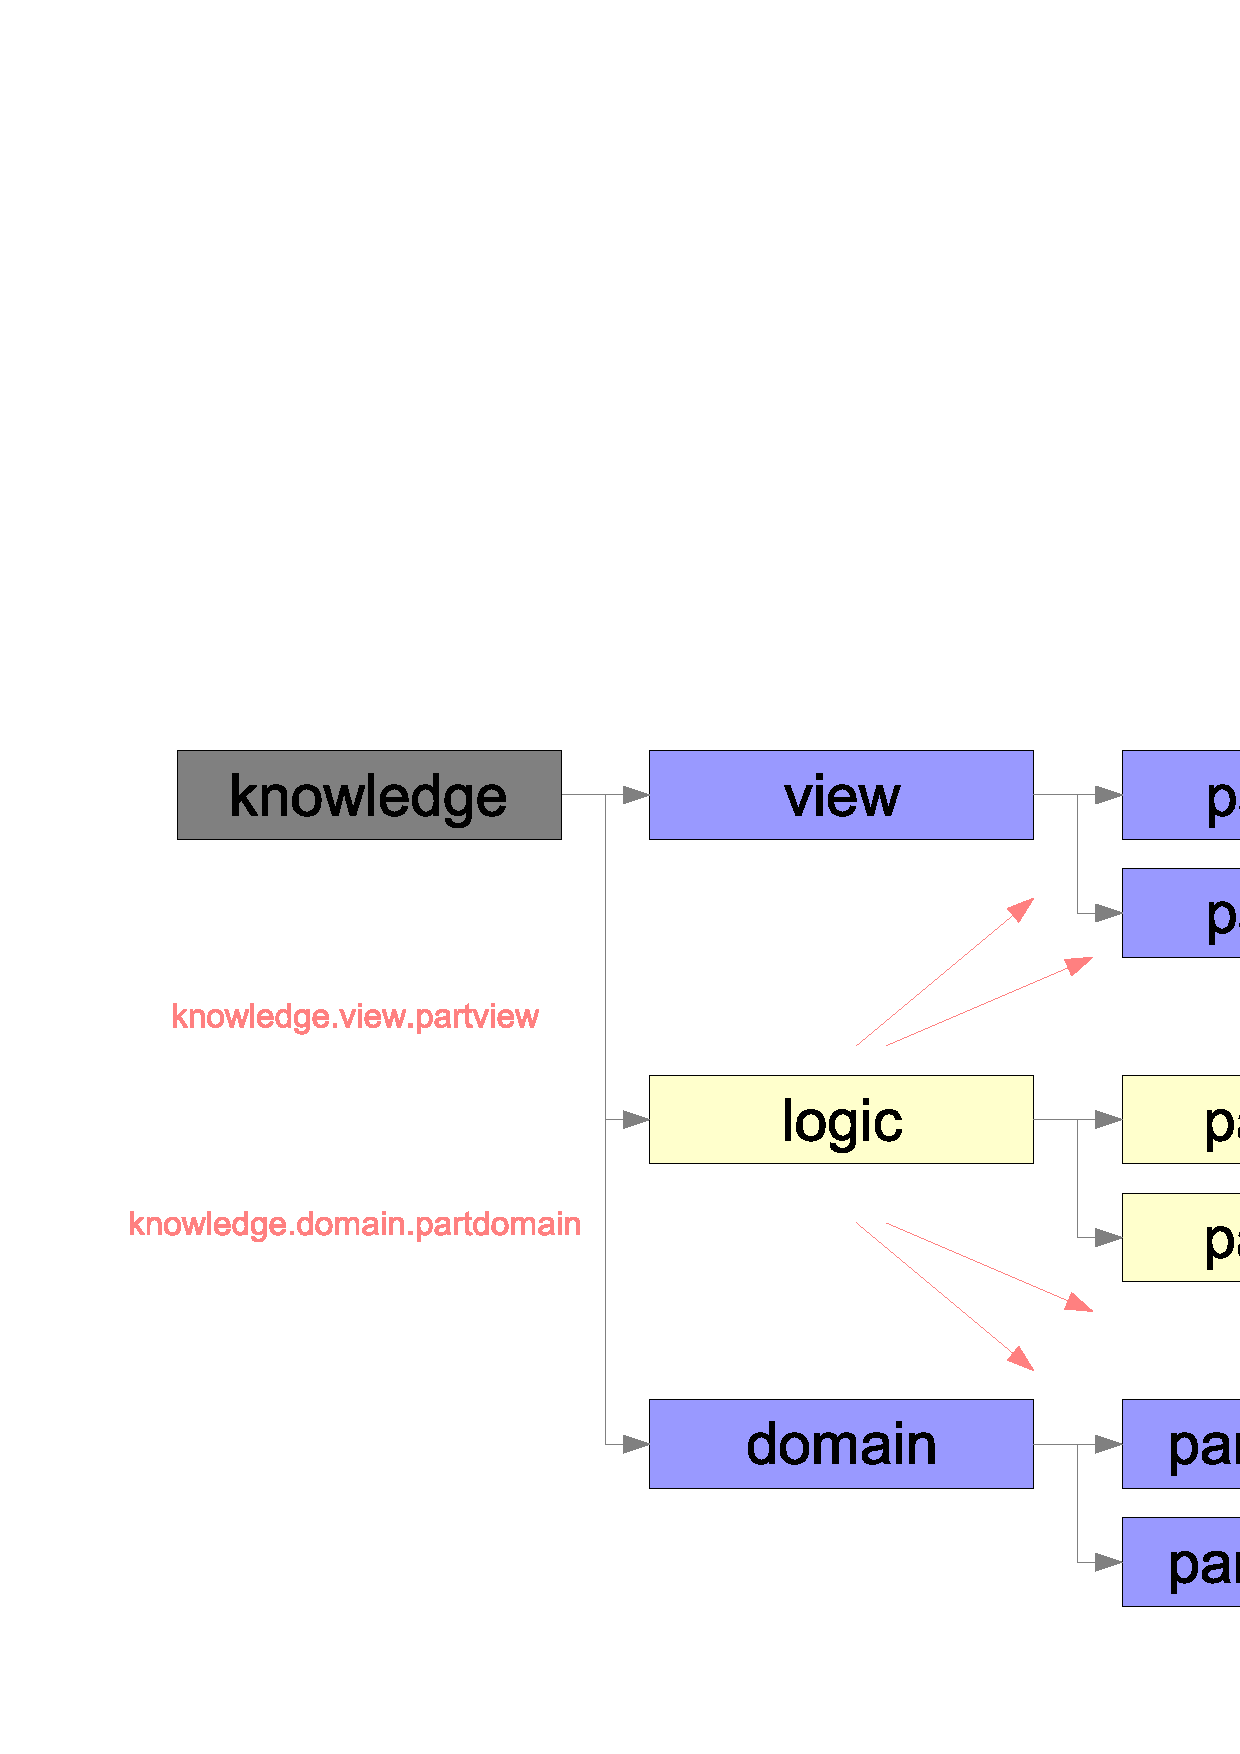
\includegraphics[scale=0.3,angle=-90]{graphic/mvctree.pdf}
        \caption{Runtime Model Hierarchy with Logic manipulating States}
        \label{mvctree_figure}
    \end{center}
\end{figure}

Figure \ref{mvctree_figure} shows the three parts: \emph{Domain} (Model),
\emph{View} and \emph{Logic} (Controller) of the MVC pattern as independent
branches of one common knowledge tree. Each of them represents a concept on its
own. The logic model, however, is allowed to access and change the view- and
domain model; it is able to link different knowledge models, to connect
discrete concepts. But view- and domain model, representing states, are not
allowed to access the logic model. In other words: The dependencies between
logic- and state models are \emph{unidirectional}. New state models such as
textual- or graphical views could be added anytime. All that would be needed to
make a system work with new state models, is the corresponding translation
logic, given in form of logic models.

Further examples may be given. A rather easy one is the \emph{Addition} of two
numbers. The corresponding knowledge model looks pretty similar to the one
shown in figure \ref{mvctree_figure}, only that there are three state models:
\emph{summand\_1}, \emph{summand\_2} and \emph{sum}. The logic model is called
\emph{add}. While being processed, the \emph{add} operation reads both summands
and writes their sum to the equally named state model. More complex examples
are the \emph{Data Mapper} and \emph{Data Transfer Object} (DTO) patterns
reflected upon in section \ref{translator_architecture_heading}. Just like the
MVC pattern, both want the same: translation for communication.

Overcoming the classical scheme of thinking in terms of \emph{Frontend},
\emph{Backend}, \emph{Domain} and \emph{Communication}, a translator-based
architecture treats them all similar, as passive data models which can be
converted into each other -- as opposed to the traditional approach and patterns
that unnecessarily complicate their handling. Translators simplify architectures
by unifying the implementation and mapping of any kind of transfer model,
thereby avoiding redundant parts. Resulting systems are highly flexible, easily
extensible and better maintainable, because the interdependency of domain
knowledge, user interface, persistence layer and (remote) communication layer
is abolished.

The clear separation of states and logic into discrete, independent models
avoids unwanted dependencies as caused by the bundling of attributes and
methods in \emph{Object Oriented Programming} (OOP) (section
\ref{classification_heading}).

One major innovation of the kind of programming suggested in this work is that
logic knowledge itself gets manipulatable. A logic model (algorithm, workflow)
cannot only access and change state-, but also logic models, and even itself!
Because models modified in that manner can be made persistent in form of CYBOL
knowledge templates (chapter \ref{cybernetics_oriented_interpreter_heading}),
and be reloaded the next time an application starts, this may be seen as a kind
of \emph{Meta Programming}, which \cite{wikipedia} defines as: \textit{the
writing of programs that write or manipulate other programs (or themselves) as
their data.}

%
% $RCSfile: without_capsules.tex,v $
%
% Copyright (C) 2002-2008. Christian Heller.
%
% Permission is granted to copy, distribute and/or modify this document
% under the terms of the GNU Free Documentation License, Version 1.1 or
% any later version published by the Free Software Foundation; with no
% Invariant Sections, with no Front-Cover Texts and with no Back-Cover
% Texts. A copy of the license is included in the section entitled
% "GNU Free Documentation License".
%
% http://www.cybop.net
% - Cybernetics Oriented Programming -
%
% http://www.resmedicinae.org
% - Information in Medicine -
%
% Version: $Revision: 1.1 $ $Date: 2008-08-19 20:41:09 $ $Author: christian $
% Authors: Christian Heller <christian.heller@tuxtax.de>
%

\subsection{Without Capsules?}
\label{without_capsules_heading}
\index{Without Capsules}
\index{Side Effect}
\index{Knowledge Tree}
\index{Encapsulation}
\index{Well-Defined Knowledge Paths}
\index{Call by Reference}
\index{Call by Value}

Once again it has to be said that all this becomes possible only because all
domain/ application knowledge is stored together in one single tree structure
which is hold and managed by the \emph{Cybernetics Oriented Interpreter}
(CYBOI) (chapter \ref{cybernetics_oriented_interpreter_heading}). What was
traditionally criticised as \emph{Side Effect}, is now a \emph{wanted} effect.
Low-level system procedures within CYBOI forward just one pointer -- the root
of the knowledge tree, which they all may access and manipulate. Data values do
\emph{not} get copied among procedures; they exist just once in the knowledge
tree and may be used by any procedure. Of course, this also means that any
application has access to the knowledge of any other application. Ways ensuring
sufficient security have to be found here (section \ref{future_works_heading}).

Besides the \emph{Encapsulation} of data through \emph{Procedures}, there are
other forms of encapsulating data, such as the \emph{Class} (section
\ref{object_oriented_programming_heading}). One of its purposes was to preserve
transient data in memory, another to restrict access to certain data. In CYBOP,
both tasks are taken care of by CYBOI. It holds the singular knowledge tree and
manages access to it, through well-defined low-level procedures.

There are a number of advantages to this style of programming: An application
developer has no chance of accessing memory areas directly, which prevents
memory leaks and wrong pointers. Because all knowledge can be accessed through
well-defined paths into the knowledge tree only, arbitrary security mechanisms
may be applied and switched as needed, at runtime. Since all algorithms (logic
knowledge) work with references to data in the knowledge tree
(\emph{Call by Reference}), no more data values need to be copied locally
(\emph{Call by Value}), which ensures efficient memory usage. Errors are not to
be expected, because nonexisting knowledge references are simply ignored by
CYBOI.

